\documentclass[11pt]{article}
\usepackage[margin=1in]{geometry}
\usepackage{graphicx}
\usepackage{booktabs}
\usepackage{amsmath}
\usepackage{xcolor}
\usepackage{hyperref}
\hypersetup{colorlinks=true, linkcolor=blue, urlcolor=blue}
\setlength{\parskip}{0.5em}
\setlength{\parindent}{0pt}
\graphicspath{{figures_solo/}}

\begin{document}

{\large \textbf{RS minimal model: floor summary and literature reproductions}}\\
{\small working notes, June 2026. Quark sector, minimal (non-custodial) Randall-Sundrum.}

\vspace{0.5em}
Quick notes after the constraint-code audit and fixes. Two things here: (1) the floor
summary (what M\textsubscript{KK} the minimal model actually needs), and (2) our reproductions
of the relevant published figures, showing just our own panel in each case. All run on the
fixed code.

\hrulefill

\section*{1. Floor summary}

There are two honest notions of a floor, and they are very different:

\begin{itemize}
\item \textbf{Typical floor:} where the \emph{median} anarchic point becomes allowed. This is
the usual literature statement. With current data it is about \textbf{30 TeV}, set by $\varepsilon_K$.
\item \textbf{Existence floor:} where even a single best-case (fine-tuned) point is allowed. This
is about \textbf{18 to 20 TeV}, set by $S,T,U$.
\end{itemize}

The split matters because the flavor constraints are tunable (you can align phases so the new-physics
piece cancels, e.g. $\varepsilon_K \propto \mathrm{Im}\,M_{12} \to 0$), but $S,T,U$ is not: in
minimal RS the oblique $T$ depends only on $M_{\rm KK}$ and the warp volume, with no Yukawa freedom.
So even a fine-tuned minimal RS point cannot sit below about 18 to 20 TeV, and that wall is the
oblique $S,T,U$ bound. This is exactly why custodial RS exists (it protects $T$).

\begin{center}
\begin{tabular}{@{}llll@{}}
\toprule
Constraint & Typical (median) floor & Existence (best/tuned) floor & Tunable? \\
\midrule
$\varepsilon_K$            & $\sim$30 TeV (current) & below $\sim$1 TeV & yes (align $\mathrm{Im}\,M_{12}\to0$) \\
$\Delta m_d$ ($B_d$)       & few TeV                & below $\sim$1 TeV & yes \\
$\Delta m_s$ ($B_s$)       & few TeV                & below $\sim$1 TeV & yes \\
$D^0$                      & low                    & below $\sim$1 TeV & yes \\
$\Delta m_K$               & low                    & below $\sim$3 TeV & yes \\
$Z\to b\bar b$ (T010)      & $\sim$5 TeV            & $\sim$4.6 TeV     & no (gauge, $c_{Q_3}$ set by $m_t$) \\
$S,T,U$ (EW001)            & $\sim$20 TeV           & $\sim$18 to 20 TeV & no (no Yukawa dependence) \\
\midrule
\textbf{Combined}          & \textbf{$\sim$30 TeV} ($\varepsilon_K$) & \textbf{$\sim$18 to 20 TeV} ($S,T,U$) & \\
\bottomrule
\end{tabular}
\end{center}

\textbf{Existence vs typical, per constraint.} Min ratio-to-bound (best, fine-tuned point) and
median ratio (typical point) vs $M_{\rm KK}$. The flavor curves crash well below 1 (tunable, no real
floor); $S,T,U$ has min $\approx$ median and crosses 1 only near 18 to 20 TeV (irreducible).

\begin{center}
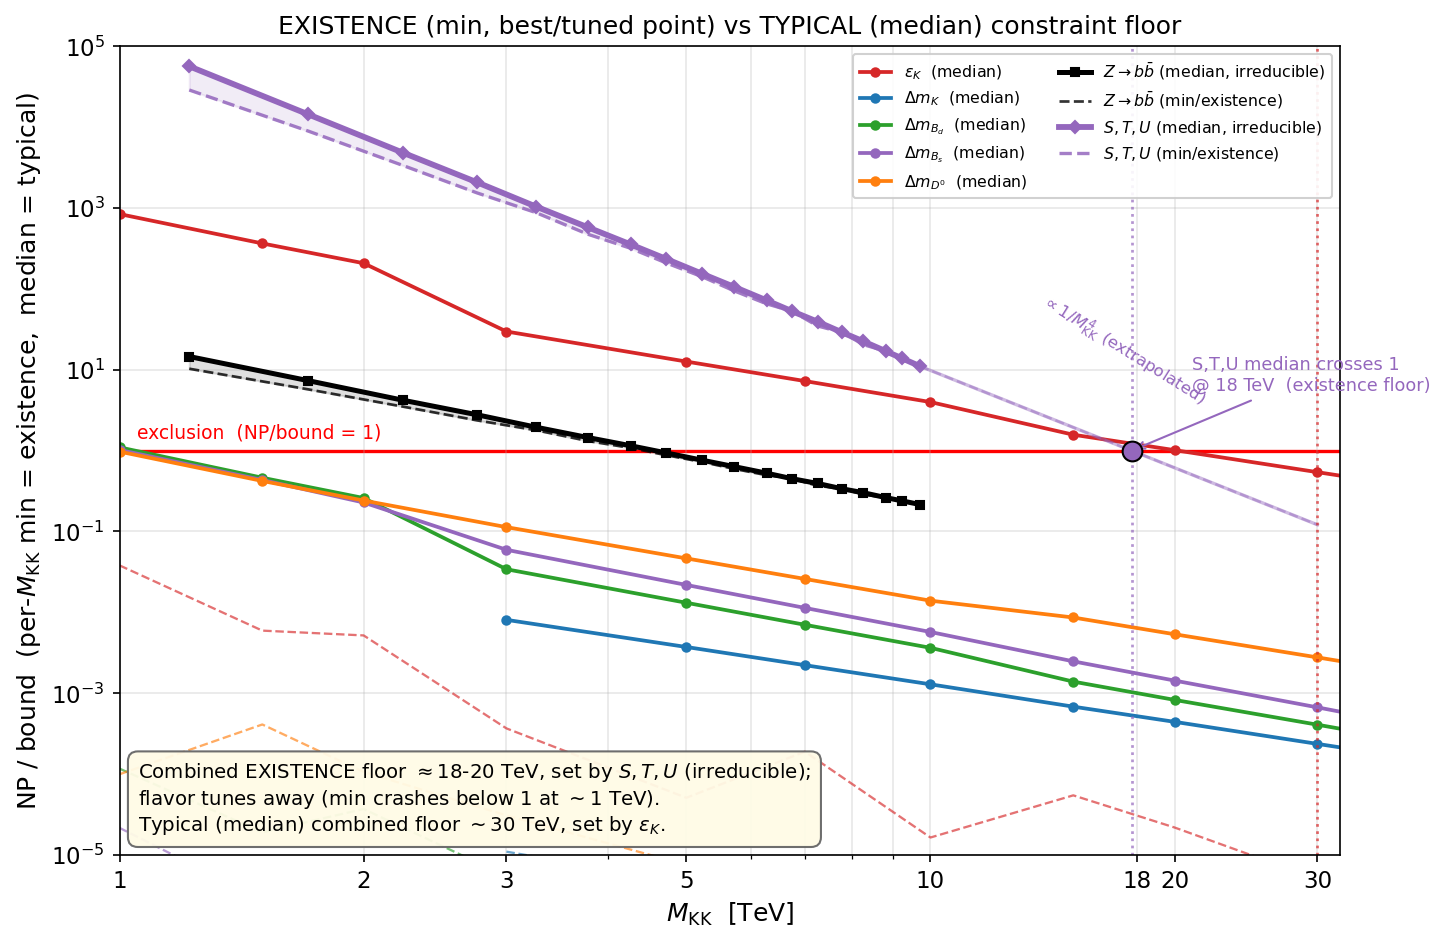
\includegraphics[width=0.86\textwidth]{solo_existence_vs_typical.png}
\end{center}

\textbf{Our 100k scan, constraint census.} Per-constraint veto fraction vs $M_{\rm KK}$ from our
minimal scan with all fixes in. Ranking: $S,T,U$ at 20, $\varepsilon_K$ at 7, $Z\to b\bar b$ at 5
(this was the old 25 to 30 TeV artifact before the fix), $\Delta m_s$ at 2. Dropping $Z\to b\bar b$
does not move the combined floor, so it is not the driver.

\begin{center}
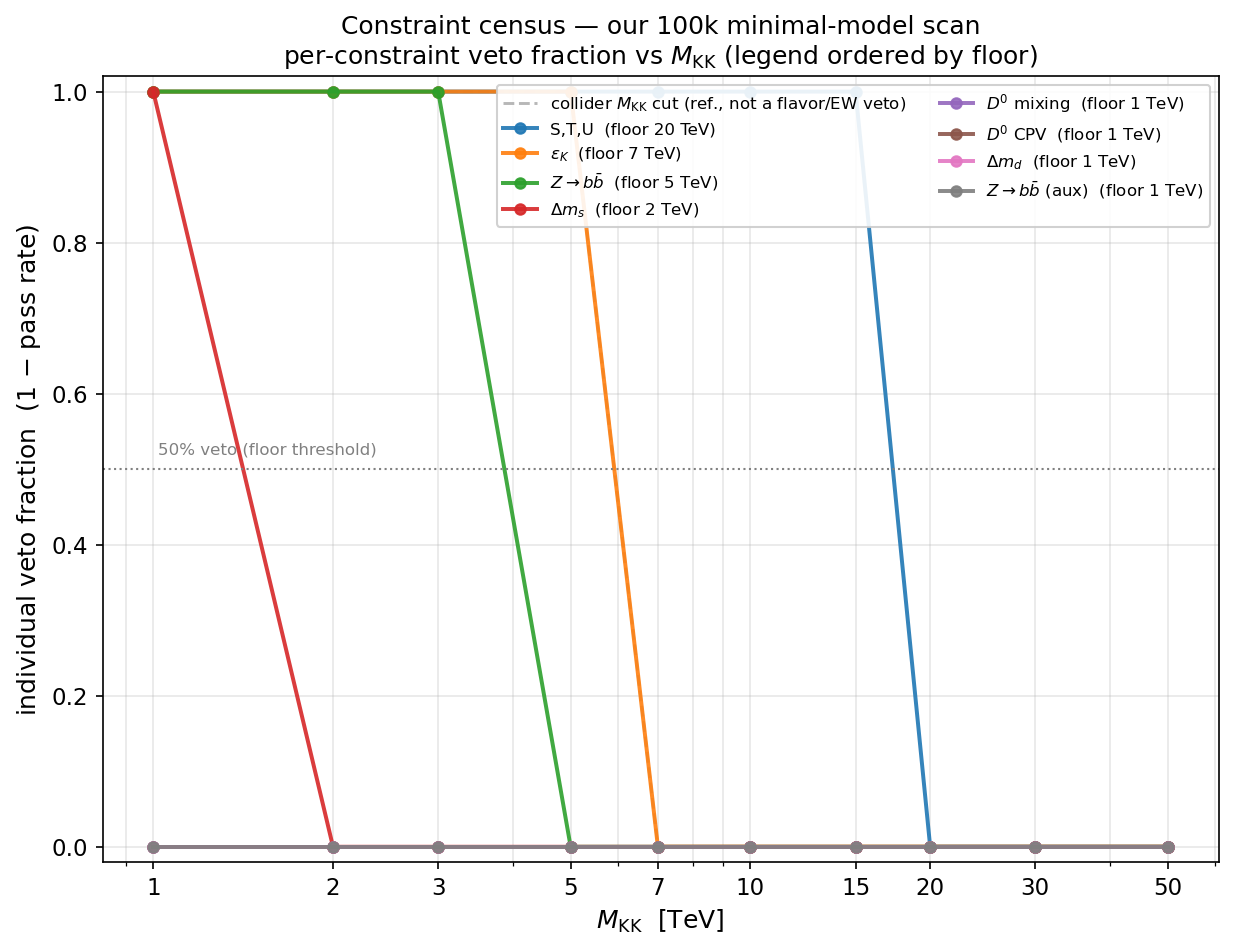
\includegraphics[width=0.92\textwidth]{solo_census.png}
\end{center}

\hrulefill

\section*{2. Reproductions (our panel only)}

For each, this is just our reproduction. The real published figure is in the longer report; here
we show only the thing we are actually reproducing.

\subsection*{$S,T,U$ oblique (vs Casagrande et al.\ 0807.4937, Fig.\ 4)}
Our $S$-$T$ plane. The RS minimal wedge climbs steeply in $T$ (the volume-enhanced $T$ problem) and
leaves our PDG-2025 ellipse fast; grey is the 2008 ellipse for reference. This is the irreducible
bound that sets the existence floor.

\begin{center}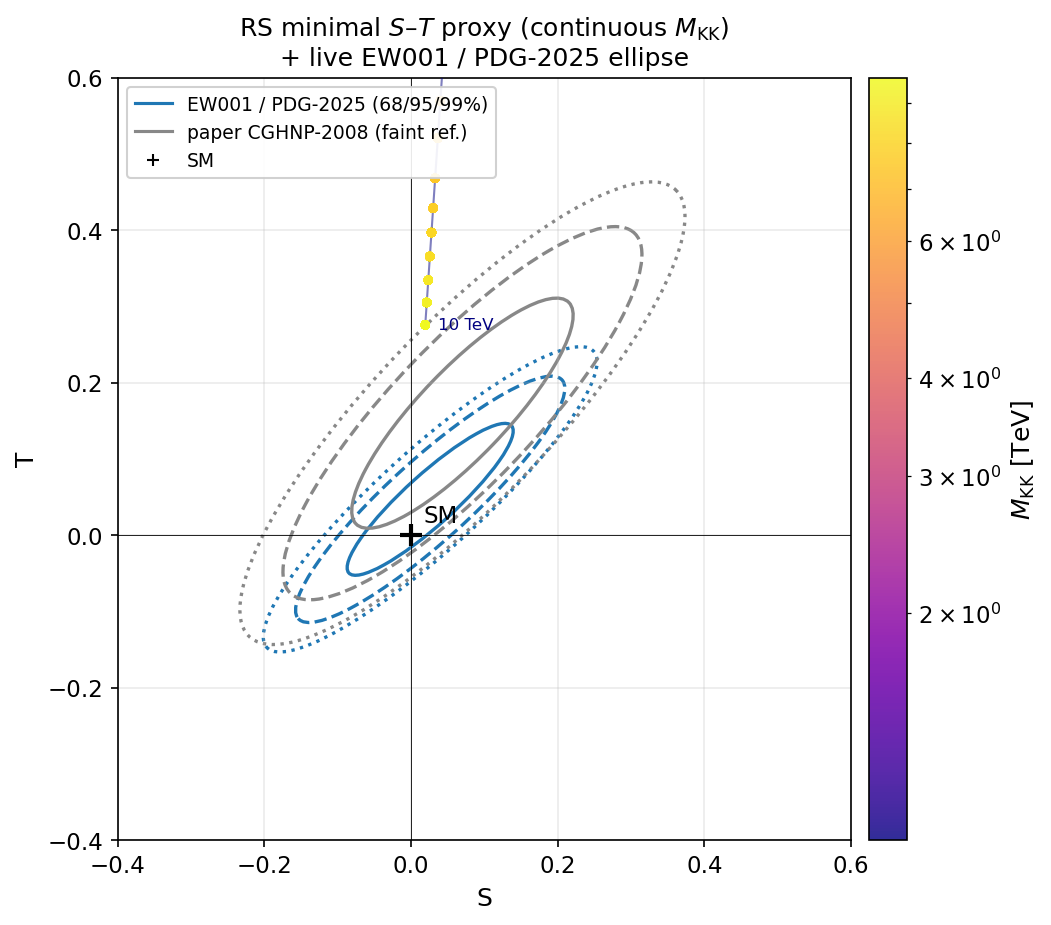
\includegraphics[width=0.72\textwidth]{solo_STU.png}\end{center}

\subsection*{$Z\to b\bar b$ couplings (vs Casagrande et al.\ 0807.4937, Fig.\ 8)}
Our $(g_L^b, g_R^b)$ plane. The RS stripe pins at $g_R^b \approx 0.077$ and slides to less-negative
$g_L^b$ as $M_{\rm KK}$ drops, staying right by the SM point. With the B1 fix this is gauge-dominated
and weak (bites only to about 5 TeV), not the 25 to 30 TeV the bug produced.

\begin{center}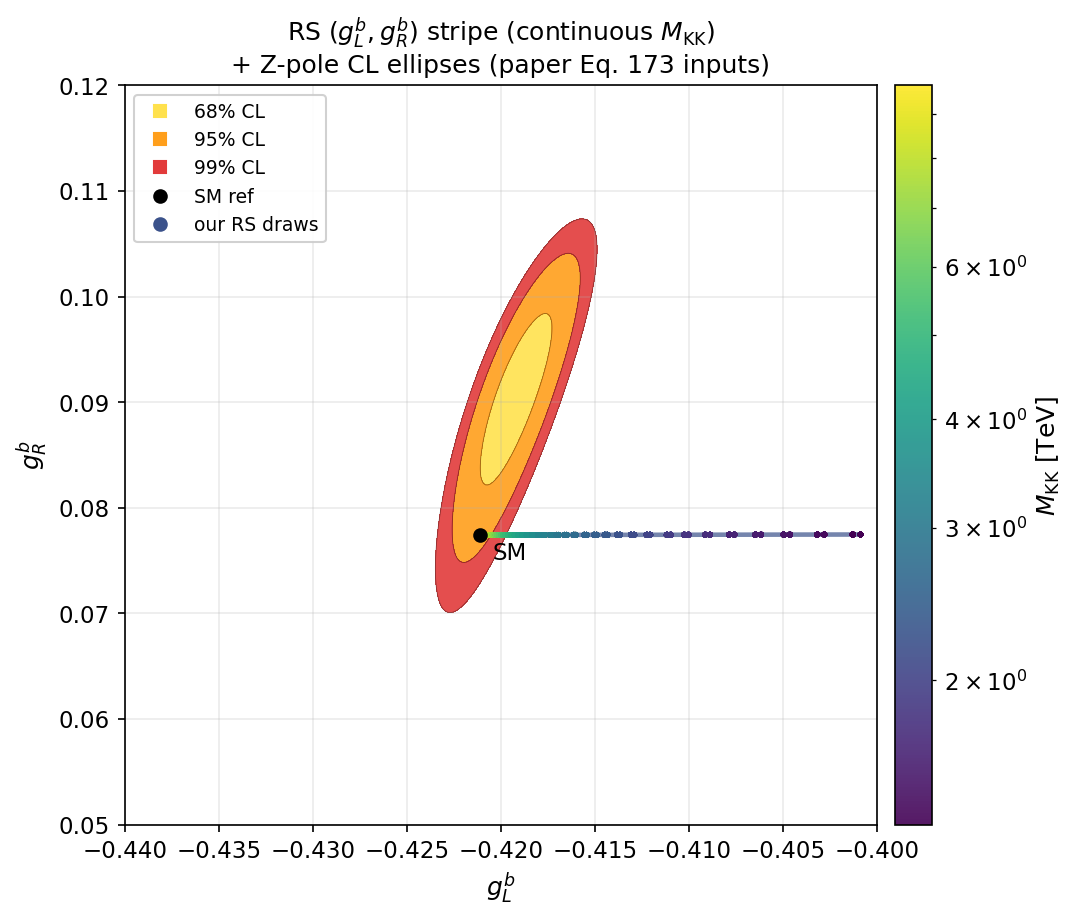
\includegraphics[width=0.72\textwidth]{solo_Zbb_gLgR.png}\end{center}

\subsection*{$\varepsilon_K$ (vs Bauer et al.\ 0912.1625, Fig.\ 4)}
Our anarchic $|\varepsilon_K|$ cloud, using Bauer's S1 draw setup ($Y_{\max}=3$, scanned $c$). Fat,
about 6 to 7 decades, with the 5/50/95 percent quantile curves. The 95 percent quantile enters the
allowed band near 10 TeV, which is Bauer's headline number.

\begin{center}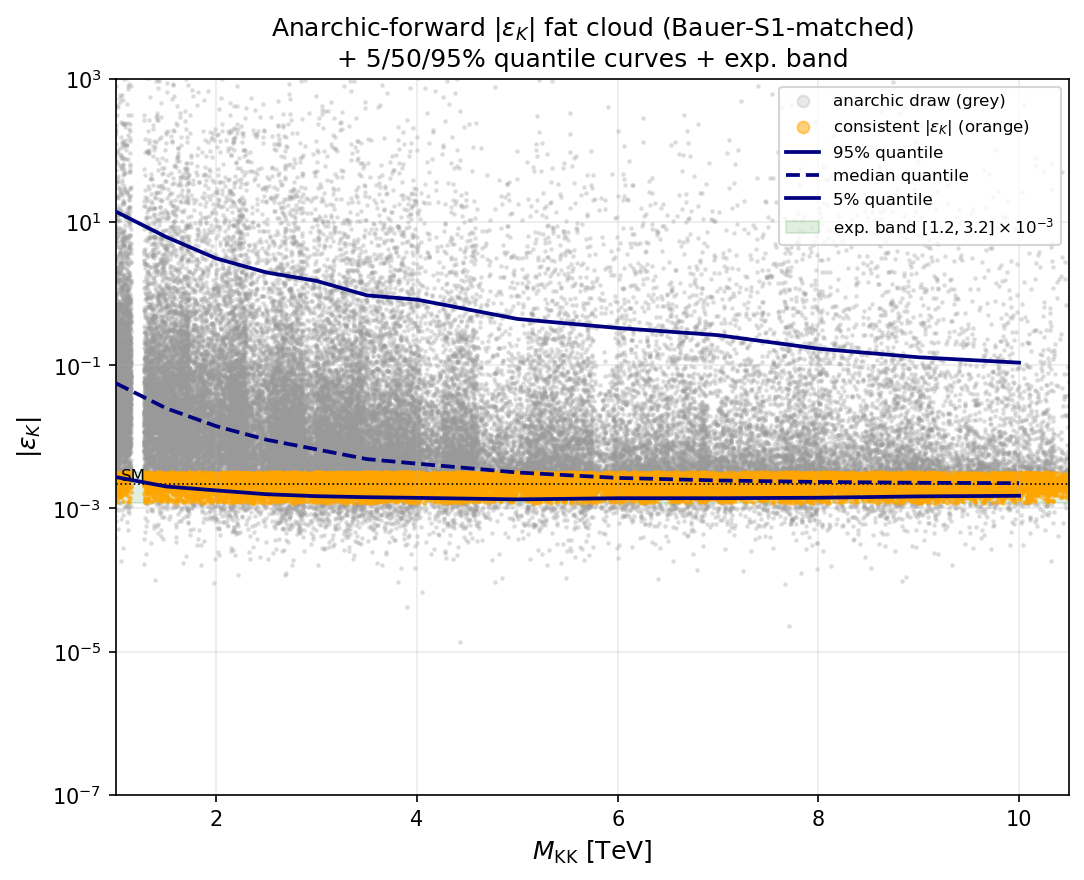
\includegraphics[width=0.74\textwidth]{solo_epsK_cloud.png}\end{center}

\subsection*{Consistency fraction (vs Bauer et al.\ 0912.1625, Fig.\ 5)}
Fraction of anarchic points consistent vs $M_{\rm KK}$, paper-era window vs current strict gate.
The rising $1/M_{\rm KK}^2$ decoupling is the same shape as the paper.

\begin{center}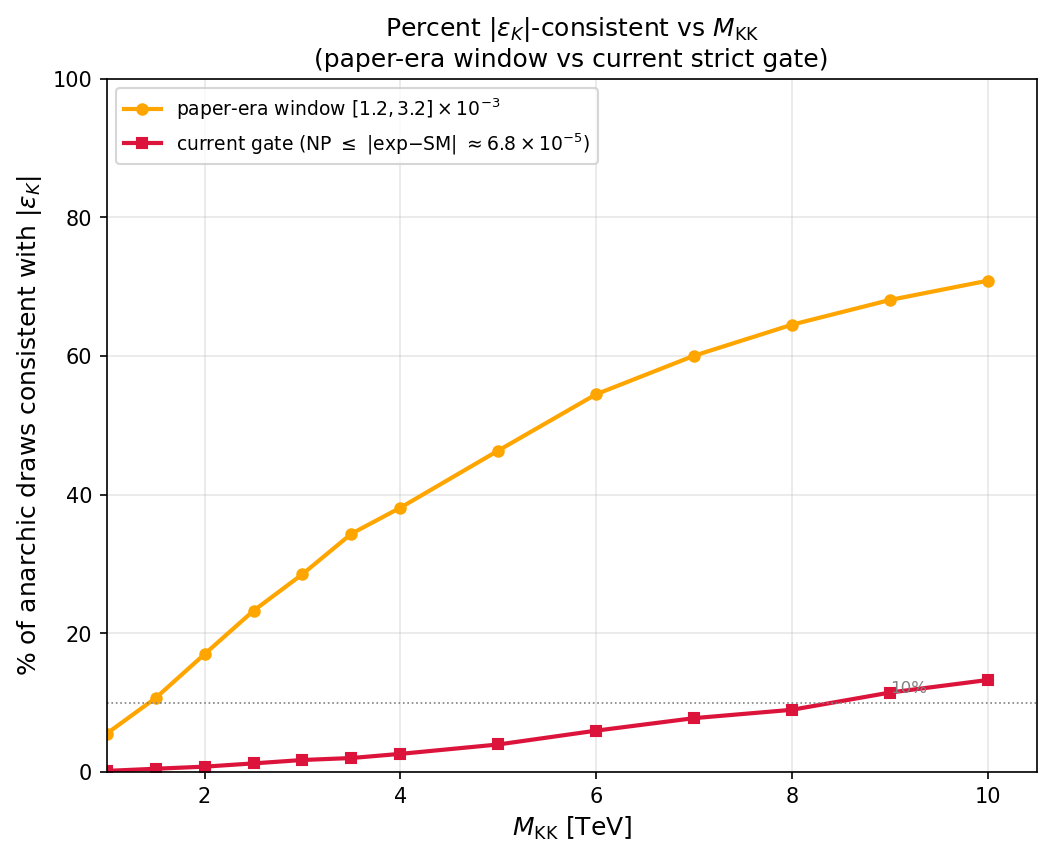
\includegraphics[width=0.7\textwidth]{solo_consistency.png}\end{center}

\subsection*{$D^0$ mixing (vs Gedalia, Grossman, Nir, Perez 0906.1879, Fig.\ 1)}
Our anarchic $D$-meson cloud on the Gedalia funnel, cleaned up to a single 3 TeV density plus the
median-$y$ trend at 1, 3, 10 TeV. The cloud sinks into the allowed funnel as $M_{\rm KK}$ rises.
(Optional figure: say the word if you would rather drop it.)

\begin{center}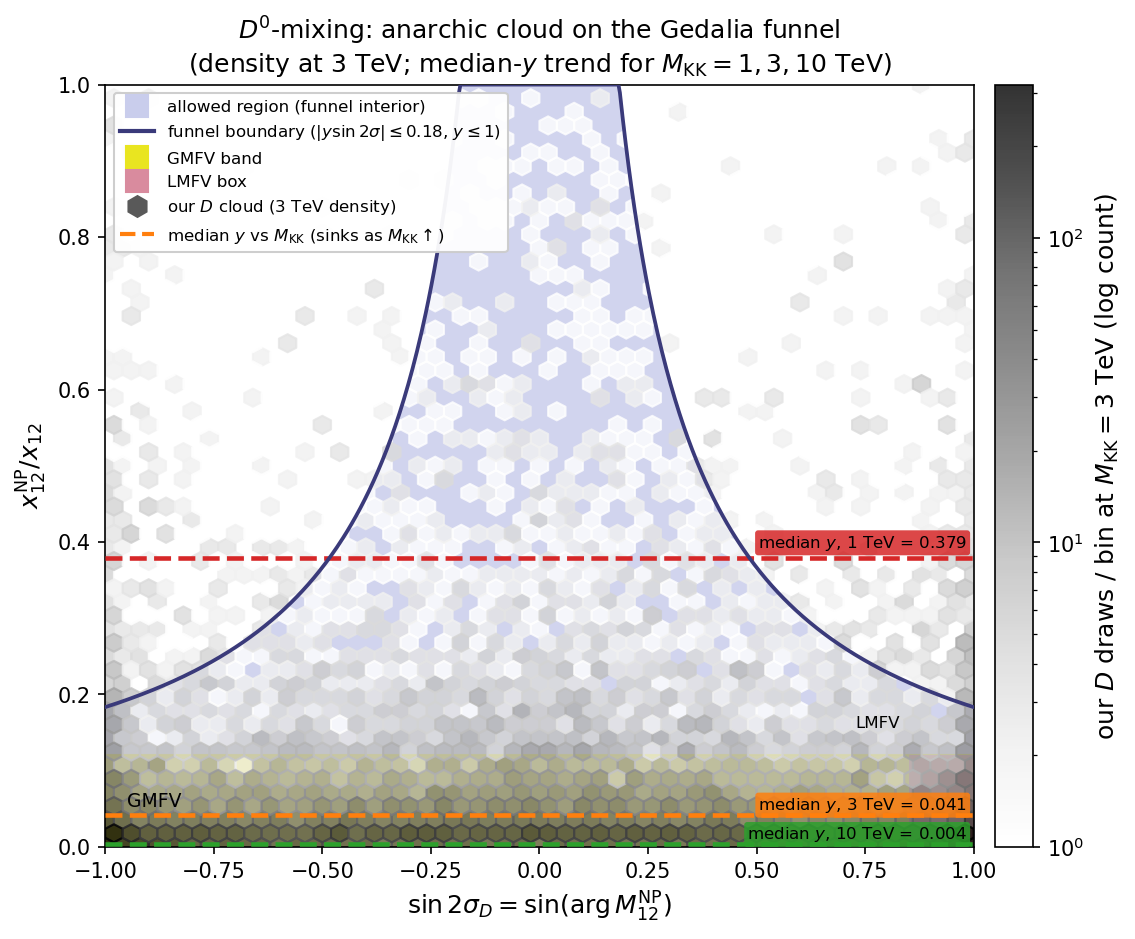
\includegraphics[width=0.72\textwidth]{solo_D0_funnel.png}\end{center}

\subsection*{$\Delta F=2$ amplitudes (vs Blanke et al.\ 0809.1073, Fig.\ 2)}
Re vs Im of the KK contribution to $M_{12}$, for $K$ (left) and $B_s$ (right). For kaons the
imaginary part dominates the real part by about $100\times$ (the $\varepsilon_K$ problem); ours is
$106\times$.

\begin{center}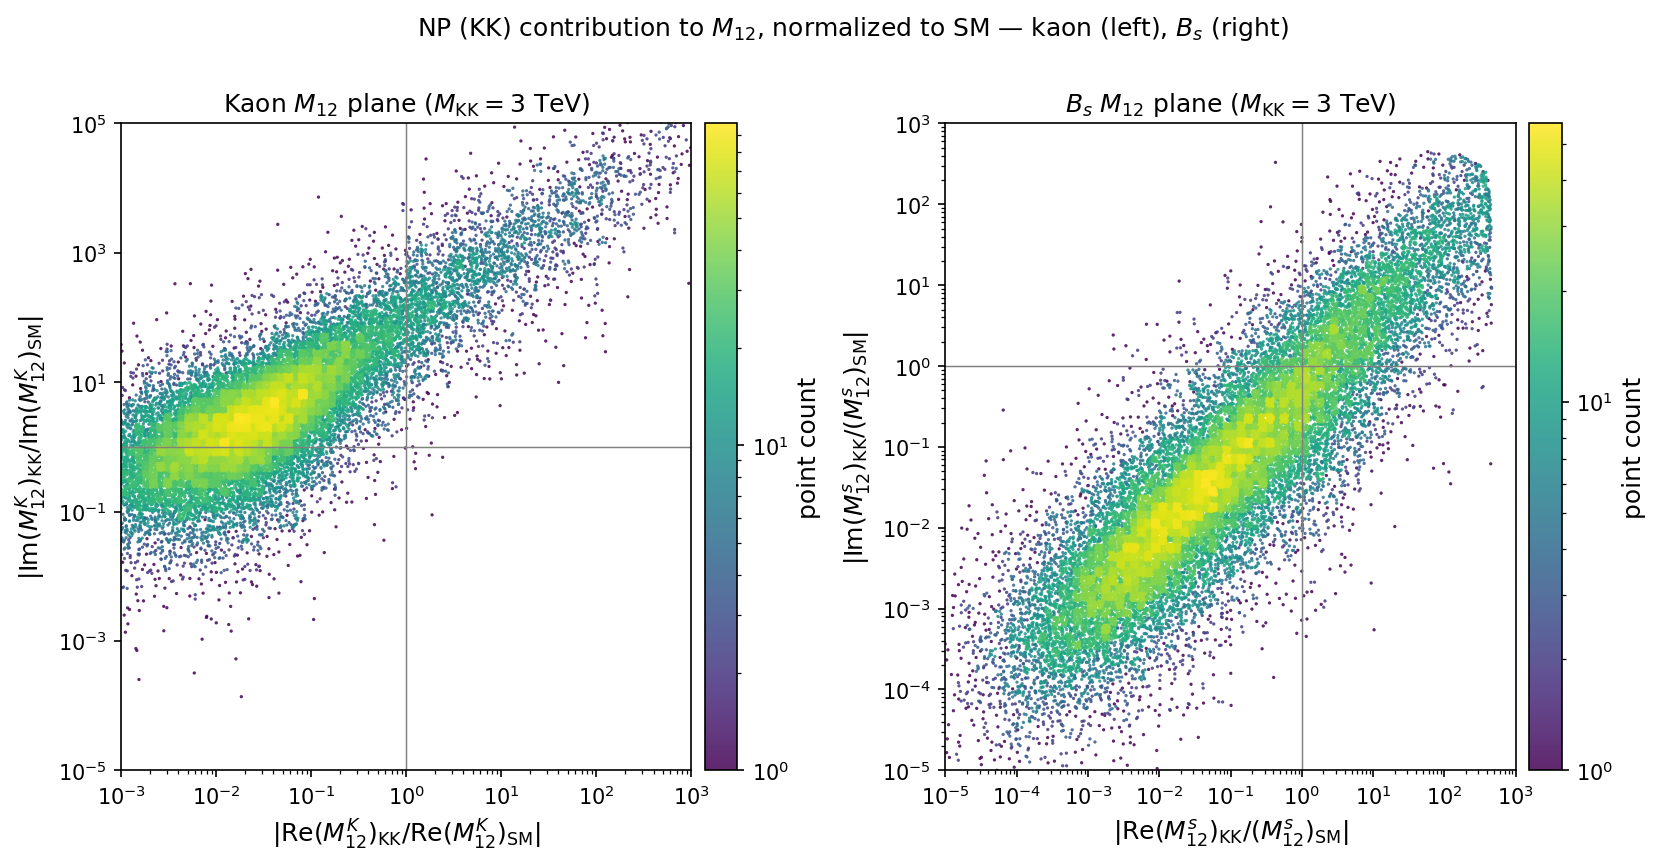
\includegraphics[width=0.92\textwidth]{solo_ReIm_M12.png}\end{center}

\vspace{0.5em}
\hrulefill

\textbf{Dropped on purpose:} the $B_d$ and $B_s$ phase planes (the old Figs 6 and 7). Our model
clouds are fine, but the experimental CL contours we drew there are only Gaussian approximations of
the CKMfitter regions, not the exact published contours, so they are not a clean reproduction. Left
out rather than shown as if exact.

\end{document}
